% 两级运载火箭发射轨迹建模与入轨优化 —— 全国大学生数学建模竞赛培训论文
% 编译：xelatex main.tex（需在模板目录内）
\documentclass[withoutpreface,bwprint]{cumcmthesis}

\usepackage{tikz}
\usepackage{cumcm2026}
\usepackage{url}
\usepackage{subcaption}

% listings 中文字体：用 xeCJK 的等宽中文字体处理，避免 lmmono 缺字
\setCJKmonofont{SimSun}[AutoFakeBold]
\lstset{
  basicstyle=\ttfamily\small,
  columns=fixed,
  keepspaces=true,
  breaklines=true,
  postbreak=\mbox{{\color{gray}$\hookrightarrow$}\space},
  commentstyle=\color{codegreen},
  keywordstyle=\color{cumcmblue}\bfseries,
  stringstyle=\color{orange!70!black},
  showstringspaces=false,
}

% 规范：摘要下为"关键词"而非"关键字"
\makeatletter
\renewcommand*{\mcm@cap@keywordsname}{关键词}
\makeatother

\title{两级运载火箭发射轨迹建模与入轨优化}

%%=======  信息（电子版不出现，占位）========
\tihao{A}
\baominghao{0000}
\schoolname{XX大学}
\membera{ }
\memberb{ }
\memberc{ }
\supervisor{ }
\yearinput{2026}
\monthinput{9}
\dayinput{1}
%===================================

\begin{document}

\maketitle

\begin{abstract}
本文研究赤道发射的两级液体运载火箭进入 400 km 圆轨道的轨迹设计问题。首先在地心惯性系中建立含地球自转、旋转大气阻力、变质量和级间质量跳变的统一动力学模型；随后按“给定控制传播—有限维参数反演—推力方向最优控制—方向与节流联合控制”的层级逐步开放决策自由度。圆轨道目标统一表示为顺行终端流形 $r=a$、$v_r=0$、$v_t=\sqrt{\mu/a}$，从而使四问共享同一物理模型和验证标准。

基准策略下，二子级燃尽时的高度、惯性速度和飞行路径角分别为 \textbf{433.53 km}、\textbf{8521.18 m/s} 和 \textbf{$-0.69^\circ$}，对应的是近地点约 431 km、远地点约 4723 km 的椭圆轨道，而非目标圆轨道。对题设恒定俯仰角速率控制，构造滑行时间、角速率和燃烧时间组成的三维非线性打靶模型，得到一组可行入轨解：滑行 \textbf{103.63 s}、角速率 \textbf{$-0.0474^\circ$/s}，剩余推进剂约 \textbf{4015 kg}。

进一步将滑行段与二级动力段转写为 Hermite--Simpson 直接配点模型，并以推进剂消耗为目标。由于问题三采用恒定满推力，最少燃料等价于最短可行燃烧时间。20/40 区间网格得到滑行时间 \textbf{4.38 s}、二级燃烧时间 \textbf{394.35 s}、推进剂消耗 \textbf{57446.93 kg}；与 10/20 网格的差异仅为 0.012 kg。所得控制经独立高精度积分复验，终端高度误差小于 1 m。问题四放开 $0.6\le\sigma\le1$ 后，正确采用累计推力积分限制推进剂容量；从满推力和 80\% 推力两类初值均收敛到 $\sigma\approx1$ 的同一候选解。因问题非凸，本文只将其称为经网格加密与独立复验支持的局部最优解，不作全局最优性保证。

\keywords{运载火箭\enspace 多阶段最优控制\enspace 直接配点\enspace 入轨打靶\enspace 推力节流}
\end{abstract}

% 目录不需要

\section{问题重述}

\subsection{问题背景}
近年来，随着深空探测与大型空间站建设需求的增加，重型运载火箭的精准入轨与推进剂优化成为航天工程的核心课题。火箭的发射过程受地球自转、重力场变化、大气阻力以及火箭自身质量不断减少等多因素协同影响。为将有效载荷以最低能量消耗送入预定轨道，必须对发射轨迹进行精准建模，并对关键飞行阶段的推力大小与方向角进行优化设计。

\subsection{已知参数与任务}
某两级液体运载火箭在赤道发射场发射，目标为将有效载荷送入高度 $H=400$ km 的近地圆轨道。火箭基本参数：一子级起飞质量 $M_0=500\,000$ kg，结构质量 $m_{s1}=40\,000$ kg，推进剂质量 $m_{p1}=380\,000$ kg，真空比冲 $I_{sp1}=300$ s，额定推力 $F_{\max1}=7.5\times10^6$ N，阻力参考面积 $S=12.5$ m$^2$，阻力系数 $C_D=0.3$；二子级结构质量 $m_{s2}=8\,000$ kg，推进剂质量 $m_{p2}=62\,000$ kg，有效载荷 $m_{pl}=10\,000$ kg，真空比冲 $I_{sp2}=420$ s，额定推力 $F_{\max2}=6.0\times10^5$ N；一子级分离后二子级气动阻力忽略；大气密度采用指数模型 $\rho(h)=1.225\,e^{-h/7200}$。

飞行过程分三个阶段：Ⅰ垂直起飞与程序转弯，一子级工作，首先垂直上升 10 s，之后推力俯仰角以恒定速度 0.4°/s 线性减小直至一子级推进剂耗尽关机分离；Ⅱ无动力滑行，二子级不点火，依靠惯性滑行设定时间；Ⅲ入轨修正，二子级点火，通过调整推力大小与俯仰角使有效载荷达到入轨条件。

需要解决以下问题：
\begin{enumerate}
    \item 建立动力学模型，在基准控制策略下仿真全程，给出高度、速度、飞行路径角与总质量曲线，并计算二子级关机时刻的轨道高度、速度与飞行路径角。基准策略为：一级额定推力；转弯段俯仰角以 0.4°/s 线性减小；二级全额推力且推力方向始终与速度方向一致；滑行时间 60 s。
    \item 设定二子级推力俯仰角以恒定速率变化，可提前关机，关机时间由入轨条件决定；调整滑行时间与俯仰角变化速率，初始俯仰角与速度方向一致，使卫星进入 400 km 近地圆轨道。
    \item 设计滑行时间与二子级推力俯仰角的优化控制策略，使二子级消耗燃料最省。
    \item 若二子级发动机具备推力节流能力，推力可在 60\%$\sim$100\% 额定推力间连续调节，重新设计滑行时间与二子级推力大小、俯仰角的优化控制策略，使燃料消耗最省。
\end{enumerate}

\section{问题分析}

\subsection{问题一的分析}
问题一要求建立物理机理模型。火箭在赤道平面内发射并进入赤道目标圆轨道，运动对称退化为平面点质量问题。关键建模要素有三：地球自转决定初速与入轨速度基准，指数大气决定阻力，阻力仰赖相对大气速度；质量流动决定推力方程与燃尽时刻。基准策略控制律确定后，问题一化为确定性的分阶段初值问题，采用高精度自适应积分并附带事件检测即可求解，重点在于物理量一致性与阶段衔接的严谨性。

\subsection{问题二的分析}
入轨条件为目标半径、零径向速度和顺行切向圆轨道速度三个等式；未知量取滑行时间、俯仰角速率和二级燃烧时间，形成三维封闭非线性打靶系统。该问只要求找到满足终端流形的参数组合，没有额外目标函数，因此所得结果是可行入轨解而非最优解。滑行段的状态预报精度会直接影响后续边值迭代质量\cite{hu2023}。

\subsection{问题三的分析}
在问题二基础上将俯仰角由单一速率参数提升为时间函数，并同时优化滑行与关机时刻。恒定满推力、恒定比冲使推进剂消耗与二级燃烧时间严格成正比，故本问的模型本质是在圆轨道终端流形上寻找最短可行燃烧时间。采用直接配点把状态方程、阶段连接和控制边界同时转写为稀疏非线性规划，可避免单重打靶把全部灵敏度压缩在终点的缺点\cite{betts1998}。

\subsection{问题四的分析}
在问题三基础上增加节流比控制量，推进剂消耗变为 $\int\sigma(t)\,dt$ 的函数。此时实际工作时间可以超过满推力燃尽时长，容量约束必须写成累计耗药量或末质量下界，不能继续限制 $t_3-t_2\le t_{b2}$。通过与问题三共用的配点模型及低节流初值同伦，检验节流是否产生真实收益；路径约束对节流结构的影响参照相关研究讨论\cite{nair2022}。

\section{模型假设}
\begin{enumerate}
    \item 火箭在赤道平面内运动，目标轨道为赤道平面内圆轨道，运动退化为平面问题；
    \item 火箭视为质点，忽略姿态动力学与攻角产生升力，只考虑推力、重力、气动阻力；
    \item 地球为均质球体，引力加速度 $\bm g=-\mu r/|r|^3$，其中 $\mu=3.986004418\times10^{14}$ m$^3$/s$^2$，地球半径取 $R_E=6371$ km；
    \item 大气随地球同步旋转，阻力使用相对地球大气速度 $v_{\rm rel}=v-\omega_E\times r$，大气密度按指数模型计算；
    \item 问题一至三的二级发动机采用额定推力，问题四允许在 60\%--100\% 范围内节流；质量流量均由真空比冲确定；
    \item 一子级分离后，二子级与有效载荷的气动阻力忽略不计；
    \item 一子级分离为瞬时事件，分离时质量发生跳变，速度位置连续；
    \item 目标圆轨道为重力场内的惯性圆轨道，入轨判据均以惯性系速度为准；
    \item 飞行动力学中推力方向始终由俯仰角控制，无侧向控制量。
\end{enumerate}

\section{符号说明}
\begin{center}
\begin{tabular}{c|p{0.4\textwidth}|c|p{0.35\textwidth}}
\toprule[1.5pt]
符号 & 含义 & 符号 & 含义 \\
\midrule[1pt]
$x,y,v_x,v_y$ & 平面惯性位置/速度分量 & $\mu$ & 地球引力常数 \\
$m$ & 当前总质量 & $R_E$ & 地球半径 \\
$r$ & 地心距 $|r|=\sqrt{x^2+y^2}$ & $\omega_E$ & 地球自转角速度 \\
$h$ & 高度 $h=r-R_E$ & $\rho$ & 大气密度 \\
$T$ & 推力大小 & $S,C_D$ & 阻力参考面积/系数 \\
$\phi$ & 推力俯仰角，与当地水平面夹角 & $I_{sp}$ & 真空比冲 \\
$\gamma$ & 飞行路径角，速度与水平面夹角 & $g_0$ & 海平面重力加速度 \\
$t_c$ & 无动力滑行时间 & $k$ & 二子级俯仰角变化率 \\
$t_1,t_2,t_3$ & 一级关机/二级点火/二级关机时刻 & $\sigma$ & 推力节流比 \\
$\bm{\hat r},\bm{\hat t}$ & 当地径向/东向单位向量 & $v_{\rm rel}$ & 相对大气速度 \\
\bottomrule[1.5pt]
\end{tabular}
\end{center}

\section{问题一：动力学模型与基准控制策略仿真}

\subsection{坐标系与状态量}
描述火箭运动的第一步是选择坐标系。火箭在赤道发射，目标为赤道平面内的圆轨道。考察发射全程的外力：重力始终指向地心，属于径向力；推力方向由俯仰角控制，本文策略中推力始终在赤道平面内；大气阻力方向与相对速度相反，只要相对速度位于赤道平面内阻力就不出该平面。初始位置在赤道平面内、初速沿赤道平面的东向，因此全部外力与初始条件均不产生垂直于赤道平面的分量，运动被约束在赤道平面内，即平面问题。

在赤道平面内采用惯性系分量描述。取发射时刻发射点所在经线为 $x$ 轴正方向，向东为 $y$ 轴正方向，$z$ 轴沿地球自转轴，则 $z$ 方向分量恒为零。记火箭地心位置向量为 $\bm r=(x,y)$，速度向量为 $\bm v=(v_x,v_y)$，当前质量为 $m$，则状态向量
\begin{equation}
\bm x=[x,\,y,\,v_x,\,v_y,\,m]^{\rm T}.
\label{eq:state}
\end{equation}
火箭在发射台上随地球自转，发射点位于赤道，地心距为 $R_E$，自转速度方向沿东向。由于 $x$ 轴选取的是发射点所在经线，发射点即位于 $x$ 轴上，故位置初值为 $(R_E,0)$；自转线速度沿 $y$ 轴方向，大小为 $\omega_E R_E$。因此初值
\begin{equation}
x(0)=R_E,\quad y(0)=0,\quad v_x(0)=0,\quad v_y(0)=\omega_E R_E,\quad m(0)=M_0.
\label{eq:ic}
\end{equation}
该初值蕴含赤道东射获得的约 465 m/s 惯性切向速度，是地球自转在发射阶段的体现。这一初速度对入轨速度基准的影响将在 §5.3 中结合入轨条件说明。

\subsection{受力分析}
火箭在飞行中受到三类外力的作用，如图 \ref{fig:forces}a 所示。

\subsubsection{推力}
发动机喷流形成推力，大小由额定推力与节流比决定。推力方向由喷管指向决定，本问题以俯仰角作为控制量，俯仰角定义为推力矢量与当地水平面的夹角。为把推力表达到惯性系，需要建立局部基向量。设当前地心位置向量为 $\bm r$，则当地径向单位向量
\begin{equation}
\bm{\hat r}=\frac{\bm r}{|\bm r|}=\left(\frac{x}{r},\frac{y}{r}\right),\qquad r=|\bm r|=\sqrt{x^{2}+y^{2}}.
\label{eq:hatr}
\end{equation}
东向单位向量 $\bm{\hat t}$ 由径向单位向量绕 $z$ 轴旋转 $90°$ 得到，
\begin{equation}
\bm{\hat t}=\left(-\frac{y}{r},\frac{x}{r}\right).
\label{eq:hatt}
\end{equation}
$\bm{\hat r}$ 与 $\bm{\hat t}$ 构成当地正交基，其中 $\bm{\hat r}$ 沿地心向外，$\bm{\hat t}$ 沿当地东向。推力矢量与 $\bm{\hat t}$ 的夹角为俯仰角 $\phi$，故推力方向单位向量
\begin{equation}
\bm{\hat u}=\cos\phi\,\bm{\hat t}+\sin\phi\,\bm{\hat r}.
\label{eq:thrustdir}
\end{equation}
$\phi=90°$ 时推力沿当地垂直方向，即垂直起飞姿态；$\phi=0$ 时推力沿水平方向。将推力大小记为 $T$，则推力向量 $\bm T=T\bm{\hat u}$，在惯性系下的分量为
\begin{equation}
T_x=T\hat u_x,\qquad T_y=T\hat u_y.
\label{eq:thrustcomp}
\end{equation}

\subsubsection{重力}
地球视为均质球体，引力场为中心引力场。引力加速度大小随地心距平方反比衰减，方向沿径向指向地心，即
\begin{equation}
\bm g=-\frac{\mu}{r^{3}}\bm r,
\label{eq:grav}
\end{equation}
其中 $\mu=3.986004418\times10^{14}$ m$^3$/s$^2$ 为地球引力常数，$r$ 为地心距。式 \eqref{eq:grav} 的直角坐标分量为
\begin{equation}
g_x=-\frac{\mu x}{r^{3}},\qquad g_y=-\frac{\mu y}{r^{3}}.
\label{eq:gravcomp}
\end{equation}
该式说明重力加速度只在近地高度范围内近似常数 $g_0$，随高度上升而减小，本题目标轨道对应重力加速度约 8.7 m/s$^2$，忽略重力随高度变化会引入不可接受的误差。

\subsubsection{气动阻力}
大气随地球同步旋转，阻力与火箭相对大气的运动有关。惯性系速度 $\bm v$ 与随地球旋转的大气速度之差为相对大气速度
\begin{equation}
\bm v_{\rm rel}=\bm v-\bm\omega_E\times\bm r.
\label{eq:vrel}
\end{equation}
在平面问题中，$\bm\omega_E\times\bm r=\omega_E(-y,\,x)$，故分量形式
\begin{equation}
v_{{\rm rel},x}=v_x+\omega_E y,\qquad v_{{\rm rel},y}=v_y-\omega_E x.
\label{eq:vrelcomp}
\end{equation}
阻力方向与相对速度方向相反，大小由动压、参考面积与阻力系数决定。动压为 $\frac{1}{2}\rho(h)|\bm v_{\rm rel}|^{2}$，其中大气密度按指数模型
\begin{equation}
\rho(h)=\rho_0\,e^{-h/h_0},\qquad \rho_0=1.225\ {\rm kg/m^3},\quad h_0=7200\ {\rm m}.
\label{eq:atmo}
\end{equation}
阻力向量为
\begin{equation}
\bm D=-\frac{1}{2}\rho(h)SC_D|\bm v_{\rm rel}|\,\bm v_{\rm rel},
\label{eq:drag}
\end{equation}
阻力在惯性系下的分量为
\begin{equation}
D_{x}=-\frac{1}{2}\rho(h)SC_D|\bm v_{\rm rel}|v_{{\rm rel},x},\qquad
D_{y}=-\frac{1}{2}\rho(h)SC_D|\bm v_{\rm rel}|v_{{\rm rel},y}.
\label{eq:dragcomp}
\end{equation}

\subsubsection{质量流出}
发动机工作时以恒定质量流量排出推进剂。真空比冲 $I_{sp}$ 定义为单位质量推进剂产生的冲量，$I_{sp}=T/(\dot m g_0)$，故质量流量
\begin{equation}
\dot m=-\frac{T}{I_{sp}\,g_0}.
\label{eq:massflow}
\end{equation}
质量流量为负表示火箭质量随时间减少。发动机关机或滑行时 $T=0$，质量保持不变。

\subsection{动力学方程}
将各外力表达式代入牛顿第二定律 $\bm F=m\bm a$，即得平面动力学方程。式 \eqref{eq:dynmass} 由式 \eqref{eq:massflow} 代入 $T=0$，式 \eqref{eq:dynx}--\eqref{eq:dyny} 右端三项依次为重力、推力与阻力加速度，分别来自式 \eqref{eq:gravcomp}、\eqref{eq:thrustcomp} 与 \eqref{eq:dragcomp}，
\begin{align}
\dot m &= -\frac{T}{I_{sp}g_0}, \label{eq:dynmass}\\
\dot x &= v_x,\qquad \dot y=v_y, \label{eq:dynkin}\\
\dot v_x &= -\frac{\mu x}{r^{3}}+\frac{T}{m}\hat u_x+\frac{D_x}{m}, \label{eq:dynx}\\
\dot v_y &= -\frac{\mu y}{r^{3}}+\frac{T}{m}\hat u_y+\frac{D_y}{m}. \label{eq:dyny}
\end{align}
其中式 \eqref{eq:dynmass} 描述推进剂消耗，质量流量由真空比冲与推力确定；式 \eqref{eq:dynkin} 为速度与位置的运动学关系；式 \eqref{eq:dynx}--\eqref{eq:dyny} 为惯性系下的动力学方程，右端三项依次为重力、推力与阻力加速度，量纲均为加速度，可直接用于积分。

飞行路径角 $\gamma$ 定义为速度向量与当地水平面的夹角，由惯性速度的径向与切向分量确定，
\begin{equation}
\gamma=\operatorname{atan2}\!\left(\bm v\cdot\bm{\hat r},
\bm v\cdot\bm{\hat t}\right).
\label{eq:gamma}
\end{equation}
图 \ref{fig:forces}a 给出坐标系与受力示意，图 \ref{fig:profile} 给出飞行剖面。

\begin{figure}[!ht]
\centering

\includegraphics[width=0.98\textwidth]{fig_forces_coords}
\caption{受力分析}
\label{fig:forces}
\end{figure}

\begin{figure}[!ht]
\centering

\includegraphics[width=0.92\textwidth]{fig_flight_profile}
\caption{飞行剖面}
\label{fig:profile}
\end{figure}

\subsection{分阶段控制策略}
按题面设定，全程划分为四个时间区间，如表 \ref{tab:q1ctrl} 所示。

\begin{table}[!htbp]
\caption{基准控制策略}
\label{tab:q1ctrl}
\centering
\begin{tabular}{c|c|c|c}
\toprule[1.5pt]
阶段 & 时间区间 & 推力 $T$ & 俯仰角 $\phi$ \\
\midrule[1pt]
垂直起飞 & $[0,10]$ s & $F_{\max1}$ & $90°$ \\
程序转弯 & $[10,t_1]$ & $F_{\max1}$ & $90°-0.4°/{\rm s}\cdot(t-10)$ \\
一子级分离 & $t_1$ & $-$ & $m\leftarrow m-m_{s1}$ \\
无动力滑行 & $[t_1,t_2]$ & $0$ & $-$ \\
二子级动力 & $[t_2, t_3]$ & $F_{\max2}$ & 与惯性速度方向一致，攻角为零 \\
\bottomrule[1.5pt]
\end{tabular}
\end{table}

一子级燃尽时刻 $t_1=m_{p1}/\dot m_1=149.06$ s，二子级燃尽时长 $t_{b2}=m_{p2}/\dot m_2=425.61$ s。滑行期 $t_c=60$ s，故 $t_2=t_1+t_c$。

\subsection{多阶段状态转移与数值验证}
全程不是一个光滑的单段常微分方程，而是由动力段、滑行段和分离跳变组成的混合动力系统。记一级动力、滑行和二级动力的状态转移分别为 $\Phi_1$、$\Phi_c$ 和 $\Phi_2$，分离质量跳变为 $\mathcal J$，则关机状态可写成
\begin{equation}
\bm x(t_3)=\Phi_2\!\left(t_3,t_2;
\mathcal J\left[\Phi_c\!\left(t_2,t_1;
\Phi_1(t_1,0;\bm x_0)\right)\right]\right).
\label{eq:phase-map}
\end{equation}
这一表达式明确了位置、速度在阶段连接处连续，而一级分离只改变质量。问题一控制律给定后，式 \eqref{eq:phase-map} 是确定的初值问题；采用自适应高阶 Runge--Kutta 方法逐段传播，并以推进剂耗尽事件截断动力段。相对容差由 $10^{-7}$ 缩小到 $10^{-11}$ 时，问题一关机高度变化小于 0.04 m、速度变化小于 $10^{-3}$ m/s，说明积分误差远小于模型误差。问题三、四的控制由直接配点求得后，再用该分段传播器独立重积分，避免把优化器内部缺陷误当成真实终端精度。

\subsection{结果与分析}
全程仿真结果如图 \ref{fig:q1res} 与表 \ref{tab:q1res} 所示。

\begin{figure}[!ht]
\centering
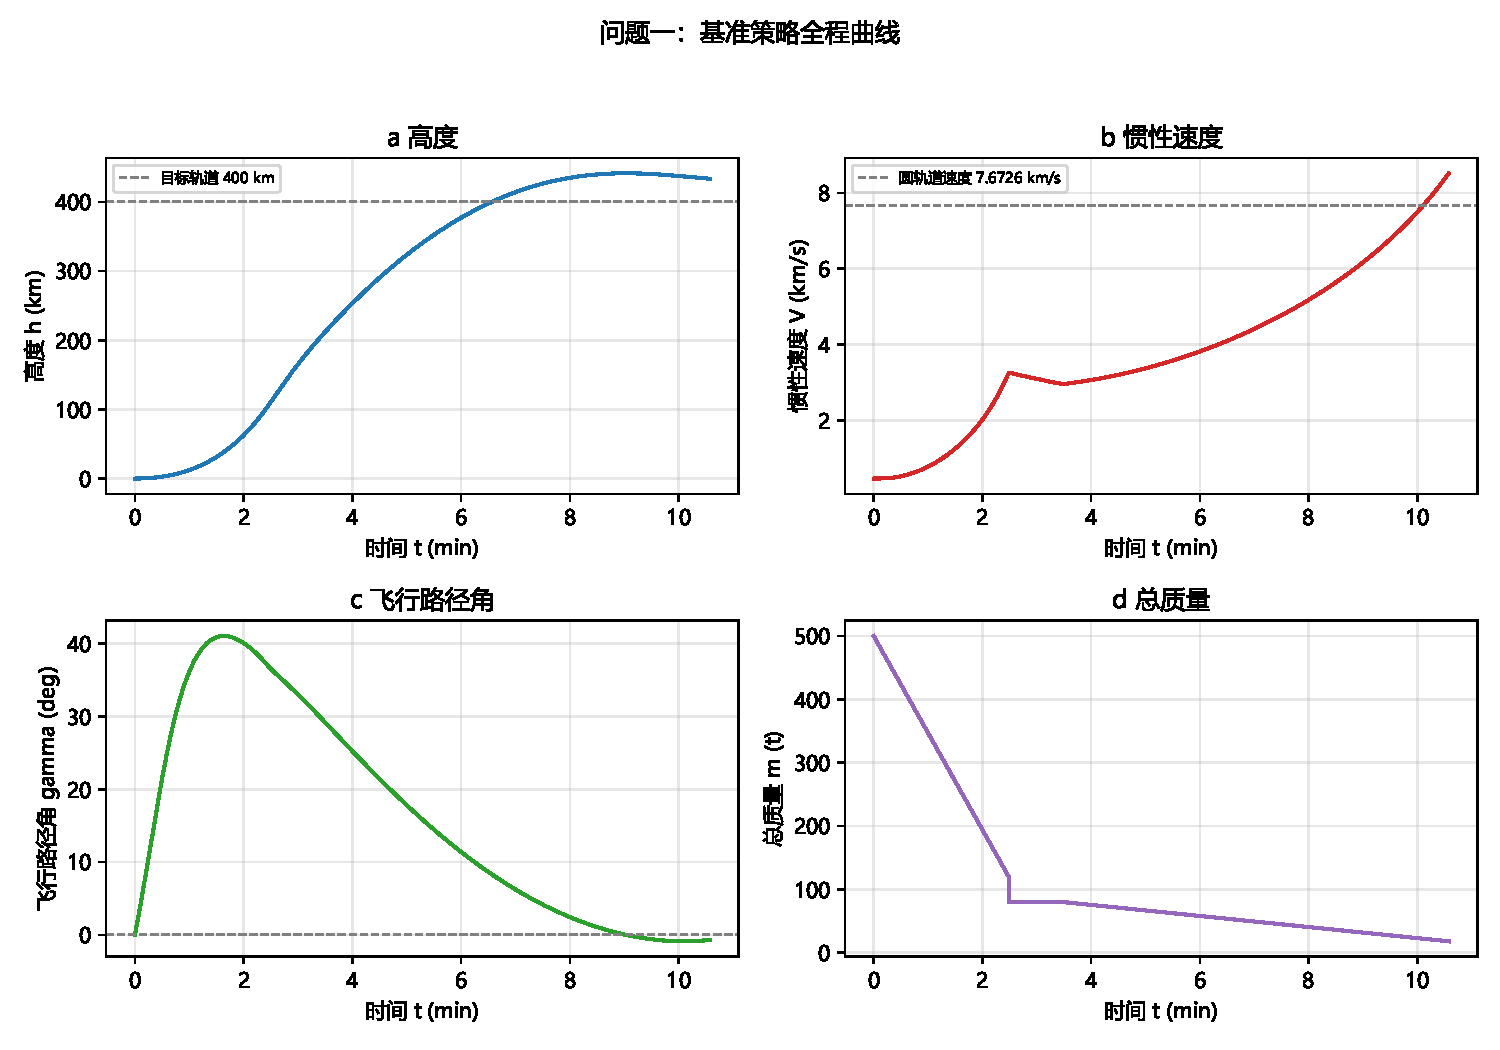
\includegraphics[width=0.92\textwidth]{fig_flight_profile2}
\caption{基准策略全程仿真曲线}
\label{fig:q1res}
\end{figure}

\begin{table}[!htbp]
\caption{全程关键结果}
\label{tab:q1res}
\centering
\begin{tabular}{c|c|c|c|c}
\toprule[1.5pt]
量 & 一子级燃尽 & 二级点火 & 二级关机 & 圆轨道目标 \\
\midrule[1pt]
时间 (s) & 149.06 & 209.06 & 634.67 & -- \\
高度 (km) & 109.26 & 210.90 & 433.53 & 400.00 \\
惯性速度 (m/s) & 3260.19 & 2954.53 & 8521.18 & 7672.60 \\
路径角 (°) & 36.61 & 29.30 & -0.69 & 0 \\
质量 (t) & 120.0 & 80.0 & 18.0 & -- \\
\bottomrule[1.5pt]
\end{tabular}
\end{table}

结果解读：
\begin{enumerate}
    \item 基准策略下二子级燃尽状态不在目标圆轨道终端流形上。由该状态反算得到半长轴约 8948 km、偏心率约 0.240，对应近地点约 431 km、远地点约 4723 km，说明它进入的是高偏心椭圆轨道，而非 400 km 圆轨道；
    \item 这印证了题面的二子级可提前关机设定，必须通过调节滑行时间、俯仰角程序与提前关机实现精确入轨；
    \item 关机速度比目标圆轨道速度高约 849 m/s，只能作为存在提前关机潜力的定性证据；实际节省量还取决于推力方向、重力损失和关机位置，不能把速度差直接等同为推进剂节省；
    \item 一子级关机点在 h=109.26 km、$\gamma=36.61°$，说明转弯段经历强重力损失与阻力损失，是后续滑行与入轨段改进的物理起点。
\end{enumerate}

\subsection{理想速度增量分析}
为量化各级实际效率，采用火箭方程计算真空理想速度增量，
\begin{equation}
\Delta v_{\rm ideal} = I_{sp1}g_0\ln\frac{M_0}{M_0-m_{p1}} + I_{sp2}g_0\ln\frac{m_{b2}}{m_{s2}+m_{pl}},
\label{eq:dv}
\end{equation}
其中 $m_{b2}=m_{s2}+m_{p2}+m_{pl}$ 为二子级点火质量。代入数值得到 $\Delta v_{\rm ideal}=10342$ m/s。而目标圆轨道惯性速度仅 7672.60 m/s，减去地球自转初速后理想增量需求为 7208 m/s。由此，两级发动机具备约 3134 m/s 的速度余量，该余量一部分被重力损失、气动阻力损失与转弯损失消耗，另一部分即提前关机留下的推进剂节约空间。这一能量关系从宏观上解释了问题二至问题四得以提前关机的物理基础，也为优化提供了判断量级。

\section{问题二：入轨条件三维打靶}

\subsection{入轨条件}
目标为半径 $a=R_E+H$ 的圆轨道。圆轨道运动的特征由角动量与机械能决定：在中心引力场中，圆轨道要求火箭在关机时刻速度方向严格沿当地切向，即径向速度为零，角动量
\begin{equation}
h=|\bm r\times\bm v|=a^2\dot\theta
\label{eq:hm}
\end{equation}
保持不变；同时，在给定半径 $a$ 处，圆轨道速度由引力与向心加速度平衡条件导出，即
\begin{equation}
\frac{\mu}{a^{2}}=\frac{v^{2}}{a}\quad\Longrightarrow\quad v=\sqrt{\frac{\mu}{a}}.
\label{eq:vcirc}
\end{equation}
因此火箭在关机时刻应满足目标半径、零径向速度与顺行切向速度三个条件。令
$v_r=\bm v\cdot\hat{\bm r}$、$v_t=\bm v\cdot\hat{\bm t}$，则
\begin{equation}
|r(t_3)|=a,\qquad v_r(t_3)=0,\qquad v_t(t_3)=+\sqrt{\mu/a}.
\label{eq:orbit3}
\end{equation}
正号排除了同样满足速度大小与正交条件的逆行圆轨道。速度在惯性系中度量，与式 \eqref{eq:ic} 的惯性初速一致。图 \ref{fig:orbit} 给出入轨条件几何关系。

\begin{figure}[!ht]
\centering

\includegraphics[width=0.85\textwidth]{fig_orbit_condition}
\caption{入轨条件}
\label{fig:orbit}
\end{figure}

\subsection{控制参数化}
二子级俯仰角以恒定速率变化，$\phi(t)=\phi_0+k(t-t_2)$，其中 $\phi_0$ 为点火时刻惯性速度路径角；$k$ 为待求变化率；推力 $T=F_{\max2}$ 恒定。为使边界清晰，以二级燃烧时间 $t_b=t_3-t_2$ 代替绝对关机时刻，未知量写为
\begin{equation}
\bm z=[t_c,\,k,\,t_b]^{\rm T}.
\label{eq:z2}
\end{equation}
该参数化方式是问题二的核心：题目指定俯仰角恒定速率变化，故俯仰角律完全由两个量决定，其一为起始值 $\phi_0$，其二为速率 $k$。而 $\phi_0$ 由点火时刻状态唯一确定，既不由优化者控制也不独立，故决策变量集合中不含 $\phi_0$。

\subsection{打靶模型}
打靶法将两点边值问题化为初值问题迭代求解。给定 $\bm z$，从已知的发射初始状态出发，依次完成垂直段、程序转弯段、分离与滑行段积分，到达二子级点火点；再按俯仰角律 $\phi(t)$ 从点火点积分至关机时刻 $t_3$，得到关机状态。该状态与目标圆轨道之间的偏差即为入轨残差。

偏差三个分量量纲不同，直接合成会掩盖小量，因此采用无量纲化形式：
\begin{equation}
F(\bm z)=\left[\frac{|r|-a}{R_E},\;
\frac{v_r}{\sqrt{\mu/a}},\;
\frac{v_t-\sqrt{\mu/a}}{\sqrt{\mu/a}}\right]^{\rm T}.
\label{eq:resid}
\end{equation}
三个分量分别对应半径偏差、速度偏差与径向速度偏差，各自以其特征量归一化，使三者处于同一量级，便于数值求解。于是问题二归结为求非线性方程组
\begin{equation}
F(\bm z)=0
\label{eq:shoot}
\end{equation}
的根。这是三个未知量对应三个独立终端条件的方阵型闭合系统；根是否存在及是否唯一需要由数值搜索与后验复验判断，不能由变量个数直接保证。

\subsection{有限维打靶与复验}
一级轨迹只计算一次；对每个 $t_c$，滑行段按二体动力学传播至二级点火，再积分二级动力段并评价 $F(\bm z)$。胡冬生等指出，滑行时间受约束时，点火状态预报精度会显著影响边值迭代质量\cite{hu2023}；在本文球形中心引力假设下，滑行段也可用 Kepler $f$--$g$ 传播替代数值积分。数值实现对三个变量设置物理边界
\begin{equation}
0\le t_c\le400\ \mathrm{s},\qquad -0.4\le k\le0.2\ ^\circ/\mathrm{s},
\qquad 0<t_b\le t_{b2},
\end{equation}
并从当前可行解附近作少量有物理意义的扰动。求得候选根后，用完整分段动力学重新传播并以米、米每秒量级的终端误差验收。求根器只是计算状态转移映射零点的工具，不构成该问的模型主体。

\subsection{结果与分析}
在给定搜索区间内得到一组通过独立复验的可行根，如表 \ref{tab:q2res} 所示。

\begin{table}[!htbp]
\caption{圆轨道入轨打靶解}
\label{tab:q2res}
\centering
\begin{tabular}{c|c|c|c|c}
\toprule[1.5pt]
滑行时间 & 变化率 & 关机时刻 & 初始俯仰角 & 剩余推进剂 \\
\midrule[1pt]
103.632 s & $-0.0474$°/s & 650.742 s & 23.128° & 4015 kg \\
\bottomrule[1.5pt]
\end{tabular}
\end{table}

入轨验证：高度 400.0000 km、惯性速度 7672.599 m/s、飞行路径角 0.0000°，残差达 $10^{-10}$ 量级。结果解读：
\begin{enumerate}
    \item 相比问题一的固定 60 s 滑行，该可行解的滑行时间增大至 103.63 s。更长的滑行使火箭在更高、更平坦的弹道上依靠重力完成转向，降低了二子级所需的方向修正量；
    \item 俯仰角变化率为轻微负值，与点火后重力转向使 $\gamma$ 自然减小的趋势匹配，避免过大攻角造成的推力浪费；
    \item 提前关机留下 4015 kg 推进剂，正是问题一过冲的修正结果。
\end{enumerate}

\subsection{滑行时间对点火状态的影响分析}
为理解最优滑行时间的分布规律，对滑行时间 0 至 300 s 扫描点火状态，结果如表 \ref{tab:tcsweep} 所示。

\begin{table}[!htbp]
\caption{滑行时间的影响}
\label{tab:tcsweep}
\centering
\begin{tabular}{c|c|c|c|c}
\toprule[1.5pt]
滑行时间 s & 点火高度 km & 惯性速度 m/s & 路径角 ° & 本地圆轨道速度差 m/s \\
\midrule[1pt]
0 & 109.26 & 3260.2 & 36.61 & 4582.6 \\
30 & 163.82 & 3098.7 & 33.12 & 4711.3 \\
60 & 210.90 & 2954.5 & 29.30 & 4827.5 \\
113 & 276.10 & 2746.1 & 21.71 & 4997.7 \\
200 & 334.25 & 2549.7 & 7.28 & 5160.4 \\
250 & 340.52 & 2527.8 & -1.64 & 5178.7 \\
300 & 327.03 & 2574.7 & -10.46 & 5139.6 \\
\bottomrule[1.5pt]
\end{tabular}
\end{table}

观察发现：滑行时间从零增大时，点火高度持续上升，路径角单调下降，在约 250 s 处路径角过零并转为负值，对应椭圆滑行弹道的远地点。继续增大滑行时间后，火箭越过远地点并开始下降。该扫描说明滑行时间同时改变点火高度、速度方向和剩余重力损失；问题二的 103.63 s 只是给定线性俯仰律下的一组可行参数，放开控制函数后最优滑行时间可以显著改变。

\section{问题三：推力方向最优控制}

\subsection{连续模型及其结构}
令 $t_b=t_3-t_2$ 为二级燃烧时间，决策对象为 $t_c$、$t_b$、状态轨迹 $\bm x(t)$ 与俯仰角函数 $\phi(t)$。标准模型为
\begin{equation}
\begin{aligned}
\min\quad &J=m(t_2^+)-m(t_3),\\
\mathrm{s.t.}\quad &\dot{\bm x}=\bm f(\bm x,\phi,F_{\max2}),\\
&r(t_3)=a,\quad v_r(t_3)=0,\quad v_t(t_3)=\sqrt{\mu/a},\\
&0\le t_c\le400\ \mathrm{s},\quad 0<t_b\le t_{b2},\\
&-90^\circ\le\phi(t)\le90^\circ,\quad
m(t)\ge m_{s2}+m_{pl}.
\end{aligned}
\label{eq:ocpq3}
\end{equation}
二级满推力且比冲恒定，故
\begin{equation}
J=\frac{F_{\max2}}{I_{sp2}g_0}t_b.
\label{eq:fuel-time-equivalence}
\end{equation}
因此，推力方向不直接改变瞬时耗药率，而是通过改变终端可行性来缩短所需燃烧时间。式 \eqref{eq:fuel-time-equivalence} 是本问最重要的结构：燃料最优问题等价为自由终端时间的最短燃烧问题。

题目只在问题二规定二级点火初始俯仰角与速度同向，问题三、四未给出姿态角速度上限；结合质点假设，本文把 $\phi(t)$ 作为可直接选取的控制量。若只固定 $\phi(t_2)$ 而不限制 $|\dot\phi|$，细网格会在点火后的极短区间形成趋于跳变的边界层，该单点条件并不能代表真实姿态连续性。因此工程化扩展应引入姿态动力学或明确约束 $|\dot\phi|\le\dot\phi_{\max}$，其数值取值需由题面或发动机摆角能力给定。

\subsection{Hermite--Simpson 直接配点}
将滑行段与二级动力段分别划分为 $N_c$ 和 $N_b$ 个区间，把每个节点的状态与控制同时作为决策变量。对任一长度为 $\Delta t$ 的区间，设端点状态为 $\bm x_k,\bm x_{k+1}$，端点导数为 $\bm f_k,\bm f_{k+1}$，中点状态采用
\begin{equation}
\bm x_{k+\frac12}=\frac{\bm x_k+\bm x_{k+1}}{2}
+\frac{\Delta t}{8}(\bm f_k-\bm f_{k+1}),
\end{equation}
并施加缺陷约束
\begin{equation}
\bm x_{k+1}-\bm x_k-
\frac{\Delta t}{6}\left(\bm f_k+4\bm f_{k+\frac12}+\bm f_{k+1}\right)=\bm0.
\label{eq:hs}
\end{equation}
由此，动力学不再隐藏在每一次目标函数评价的黑箱积分中，而是成为稀疏非线性规划的显式约束；阶段连接、质量下界和终端流形也以同一方式进入模型。该结构与 YAPSS Delta III 算例中的多阶段连续动力学、阶段连接和终端约束思想一致\cite{yapss}，但本文针对题设重新建立了两级质量、滑行时间和节流约束。直接法与打靶法的适用特点可参见 Betts 的综述\cite{betts1998}，更高阶伪谱离散可作为扩展\cite{liu2019}。

为改善尺度，以 $a$、$\sqrt{\mu/a}$ 和 80000 kg 分别无量纲化位置、速度与质量。用问题二的可行轨迹作为初值，利用 CasADi 自动微分和内点法求解式 \eqref{eq:hs} 形成的稀疏规划\cite{casadi}；求解结束后，将节点控制作分段线性插值，并用与配点过程独立的高精度积分器重新传播。这里数值算法只负责求解离散后的数学模型，可靠性由网格加密和独立复验共同判断。

\subsection{结果与网格一致性}
表 \ref{tab:q3res} 给出两级网格结果。20/40 网格的关机时刻为 $t_3=547.791$ s，剩余推进剂为 4553.07 kg；俯仰角由点火时约 $7.31^\circ$ 平滑降至约 $1.71^\circ$，末段回升至 $2.27^\circ$，用于同时消除径向速度误差并补足切向速度。

\begin{table}[!htbp]
\caption{问题三配点网格加密与独立复验}
\label{tab:q3res}
\centering
\begin{tabular}{c|c|c|c|c|c}
\toprule[1.5pt]
$(N_c,N_b)$ & 滑行时间/s & 燃烧时间/s & 耗药/kg & 高度误差/m & $(\Delta v_r,\Delta v_t)$/m/s \\
\midrule[1pt]
$(10,20)$ & 4.37665 & 394.35331 & 57446.923 & $-0.668$ & $(-0.0022,-0.0015)$ \\
$(20,40)$ & 4.37670 & 394.35339 & 57446.934 & $-0.919$ & $(-0.0073,\phantom{-}0.0010)$ \\
\bottomrule[1.5pt]
\end{tabular}
\end{table}

两级网格耗药差为 0.012 kg，说明目标值已基本稳定；独立传播的终端高度误差小于 1 m，径向和切向速度误差均小于 0.01 m/s。与问题二线性俯仰律相比，耗药减少约 538.4 kg。更重要的是，滑行时间从 103.63 s 改变为约 4.38 s，表明旧的低维控制参数限制了可行轨迹族；这不是更换求解器本身带来的收益，而是连续推力方向模型释放了新的控制自由度。由于该问题非凸，本文将表中结果称为经过网格一致性检验的局部最优候选解，不宣称全局最优。

\section{问题四：推力节流下的燃料最省优化}

\subsection{节流模型与推进剂约束}
在问题三中增加节流比 $\sigma(t)$，使
\begin{equation}
T(t)=\sigma(t)F_{\max2},\qquad
\dot m=-\frac{\sigma(t)F_{\max2}}{I_{sp2}g_0},qquad
0.6\le\sigma(t)\le1.
\end{equation}
目标函数为
\begin{equation}
J(\bm z)=\int_{t_2}^{t_3}\frac{\sigma(t)F_{\max2}}{I_{sp2}g_0}\,dt=m(t_2^{+})-m(t_3).
\label{eq:obj4}
\end{equation}
问题四与问题三的关键区别在于：满推力燃尽时长 $t_{b2}=425.61$ s 不再是实际工作时间的上界。例如恒定 60\% 推力使用全部推进剂可工作 $t_{b2}/0.6\approx709.35$ s。因此正确的容量约束是
\begin{equation}
\int_{t_2}^{t_3}\sigma(t)\,dt\le t_{b2},
\quad\Longleftrightarrow\quad
m(t_3)\ge m_{s2}+m_{pl}=18000\ \mathrm{kg}.
\label{eq:q4-fuel-capacity}
\end{equation}
采用式 \eqref{eq:q4-fuel-capacity} 后，低推力长燃烧轨迹不会被人为排除。其余动力学、阶段连接和顺行圆轨道终端条件与问题三完全相同。

\subsection{与问题三共用的配点转录}
在每个二级动力节点增加 $\sigma_k$，并将式 \eqref{eq:hs} 中的推力与质量流量替换为节流形式，即可复用同一套 Hermite--Simpson 转录。先以问题三的 $\sigma\equiv1$ 解暖启动，再以 $\sigma\equiv0.8$、燃烧时间相应延长的轨迹作为独立初值。两类初值均在同一物理可行域内求解，避免依靠几十组盲目初值暴力搜索。

\subsection{结果与分析}
结果如表 \ref{tab:q4res} 所示。40 区间节流节点全部位于 $0.99999$ 至 1.00000，低节流初值也回到同一满推力候选解。

\begin{table}[!htbp]
\caption{问题四配点结果与独立复验}
\label{tab:q4res}
\centering
\begin{tabular}{c|c|c|c|c|c}
\toprule[1.5pt]
$(N_c,N_b)$ & 滑行时间/s & 燃烧时间/s & 节流范围 & 耗药/kg & 高度误差/m \\
\midrule[1pt]
$(10,20)$ & 4.37651 & 394.35350 & 0.999993--1 & 57446.923 & $-0.898$ \\
$(20,40)$ & 4.37641 & 394.35381 & 0.999999--1 & 57446.935 & $-0.005$ \\
\bottomrule[1.5pt]
\end{tabular}
\end{table}

\subsection{物理解释与文献对照}
在固定比冲模型中，降低推力会延长发动机在重力场中的工作时间，通常增加重力损失；本题又没有最大动压、过载或热流等迫使发动机降推力的路径约束，因而数值解落在满推力边界具有明确物理解释。Nair 与 Vaidyanathan 的研究表明，节流的重要价值常来自满足路径约束并重塑整体弹道\cite{nair2022}。然而，本文的两种初值和两级网格仍只是局部数值证据，不能推出“无路径约束时节流必然无收益”的一般定理；若要作此断言，还需对 Hamilton 函数关于 $\sigma$ 的切换函数符号给出严格证明。

\section{模型评价}

\subsection{优点}
\begin{enumerate}
    \item 坐标系处理一致：运动方程写在地心惯性系中，地球自转同时进入初始速度与旋转大气相对速度，避免混用惯性速度和相对速度；
    \item 四问共享同一多阶段动力学和顺行圆轨道终端流形，只逐步开放控制自由度，因而不同问题的结果可以直接比较；
    \item 问题三揭示了“恒定满推力下最少燃料等价于最短燃烧时间”的结构，问题四则把容量条件正确提升为累计推力积分约束；
    \item 配点控制均由独立初值问题积分器复验，并给出网格加密、米级高度误差和米每秒级速度误差，区分了离散模型可行性与真实动力学可行性。
\end{enumerate}

\subsection{缺点与改进}
\begin{enumerate}
    \item 平面假设忽略侧向运动，若目标轨道含倾角或发射场不在赤道，需扩展为三维模型；
    \item 采用球形中心引力、指数大气和恒定比冲，地球半径取 6371 km；若改用赤道半径或加入 $J_2$，数值结果会发生系统变化，应做常数与模型敏感性分析；
    \item 直接配点得到的是非凸规划的局部最优候选解。网格一致性与不同初值提高可信度，但不等同于全局最优证明；
    \item 未考虑最大动压、过载、热流、俯仰角速度等路径约束。加入这些约束后，节流可能出现非平凡切换结构，应重新求解而不能沿用本问结论\cite{nair2022,benedikter2022}；
    \item 可进一步采用高斯伪谱法\cite{liu2019}或三维制导模型\cite{li2023}进行交叉验证。
\end{enumerate}

\section{结论}
本文以统一的多阶段变质量动力学为主线回答四问。问题一表明基准策略将火箭送入高远地点椭圆轨道而非目标圆轨道；问题二在题设线性俯仰律下给出一组精确可行的三变量打靶解。问题三放开推力方向函数后，直接配点候选解将滑行时间缩短到约 4.38 s，耗药量降至 57446.93 kg，网格加密差异约 0.012 kg。问题四采用正确的累计耗药约束后，从满推力和低推力初值均收敛到近似满推力控制，在当前模型和网格下未发现节流收益。上述第三、四问结论均经独立高精度传播复验，但鉴于问题非凸，只作局部最优性陈述。该分层建模方式也符合运载火箭总体弹道设计由任务约束逐级落实到控制变量的基本思路\cite{yu2023}。

\begin{thebibliography}{9}%宽度9
\bibitem[1]{nair2022}
Nair V S, Vaidyanathan A. Ascent trajectory design and optimization of a two-stage throttleable liquid rocket[J]. Advances in Space Research, 2022, 69(12): 4358--4375.
\bibitem[2]{benedikter2022}
Benedikter B, Zavoli A, Colasurdo G, et al. Convex optimization of launch vehicle ascent trajectory with heat-flux and splash-down constraints[J]. Journal of Spacecraft and Rockets, 2022, 59(3): 900--915.
\bibitem[3]{betts1998}
Betts J T. Survey of numerical methods for trajectory optimization[J]. Journal of Guidance, Control, and Dynamics, 1998, 21(2): 193--207.
\bibitem[4]{liu2019}
刘超越, 张成. 基于高斯伪谱法的二级助推战术火箭多阶段轨迹优化[J]. 兵工学报, 2019, 40(2): 292--302.
\bibitem[5]{hu2023}
胡冬生, 刘楠, 童科伟, 等. 含滑行时间约束的真空段弹道设计研究[J]. 宇航总体技术, 2023, 7(1): 14--20.
\bibitem[6]{li2023}
李惠峰, 张冉, 王嘉炜. 液体火箭上升段制导方法的发展综述[J]. 航天控制, 2023, 41(4): 3--12.
\bibitem[7]{yu2023}
余梦伦, 刘银, 张志国. 弹道学在运载火箭总体设计中的实践与展望[J]. 宇航总体技术, 2023, 7(2): 13--22.
\bibitem[8]{casadi}
Andersson J A E, Gillis J, Horn G, et al. CasADi: a software framework for nonlinear optimization and optimal control[J]. Mathematical Programming Computation, 2019, 11: 1--36. \url{https://web.casadi.org/docs/#optimal-control-with-casadi}.
\bibitem[9]{yapss}
YAPSS Documentation. Delta III launch vehicle ascent problem[EB/OL]. \url{https://yapss.readthedocs.io/en/stable/notebooks/delta_iii_ascent.html}.
\end{thebibliography}

\end{document}
